% Created with jtex v.1.0.20
%%%%%%%%%%%%%%%%%%%%%%%%%%%%%%%%%%%%%%%%%%%%%%%%%%%%%%%%%%%%
%%% LaPreprint: PREPRINT TEMPLATE
%%%%%%%%%%%%%%%%%%%%%%%%%%%%%%%%%%%%%%%%%%%%%%%%%%%%%%%%%%%%

% Here I could talk about what one should do in this document.
% Instead I'll refer you to the explore on your own and check the Github Repo. :-)
% Line spacing is 1.2 by default (can't be smaller).

%%%%%%%%%%%%%%%%%%%%%%%%%%%%%%%%%%%%%%%%%%%%%%%%%%%%%%%%%%%%
%%% PREAMBLE
%%%%%%%%%%%%%%%%%%%%%%%%%%%%%%%%%%%%%%%%%%%%%%%%%%%%%%%%%%%%

% Declare document class
\documentclass[9pt,Preprint]{lapreprint}
% Choose between "biorxiv", "medrxiv", "arxiv" and "chemrxiv". Otherwise defaults "Preprint".
% Choose between "blue" and "red" colour scheme. Defaults to "blue".
% Use the "onehalfspacing" option for 1.5 line spacing.
% Use the "doublespacing" option for 2.0 line spacing.
% Use the "lineno" option for line numbers.
% Use the "endfloat" option to place floats after the bibliography.
% Use the "secnum" option to have include numbers.

% Import packages
% \usepackage{lipsum}     % Required to insert dummy text
\usepackage[version=4]{mhchem} % For chemical notation
\usepackage{siunitx}    % For SI units
\usepackage{pdflscape}  % For putting pages in landscape mode
\usepackage{rotating}   % For rotating specific elements
\usepackage{textgreek}  % Greek symbols
\usepackage{gensymb}    % Symbols
\usepackage[misc]{ifsym} % For the \Letter symbol
\usepackage{orcidlink}  % For the \orcidlink
\usepackage{listings}   % For inserting code chunks
\usepackage{colortbl}   % For Knitr table colouring
\usepackage{tabularx}   % For making Knitr tables compatible
\usepackage{longtable}  % For multi-page tables
\usepackage{subcaption}
\usepackage{multirow}
\usepackage{snotez}     % For sidenote environments. enotez for endnotes
\usepackage{csquotes}   % For language-based quote rules (helps BiBLaTeX)



% Make declarations
\DeclareSIUnit\Molar{M}

% Please note that these options may affect formatting.

%%%%%%%%%%%%%%%%%%%%%%%%%%%%%%%%%%%%%%%%%%%%%%%%%%%%%%%%%%%%
%%% BIBLIOGRAPHY
%%%%%%%%%%%%%%%%%%%%%%%%%%%%%%%%%%%%%%%%%%%%%%%%%%%%%%%%%%%%
\usepackage[			% use biblatex for bibliography
	backend=biber,      % use biber or bibtex backend
    style=authoryear,   % choose style
	natbib=true,		% allow natbib commands
	hyperref=true,	    % activate hyperref support
	alldates=year,      % only show year (not month)
]{biblatex}

% Just avoiding some rogue fields that cause issues with certain styles
\AtEveryBibitem{
    \clearfield{urlyear}
    \clearfield{urlmonth}
    \clearlist{language}
}

% Update to your bibliography file
\addbibresource{main.bib}


%%%%%%%%%%%%%%%%%%%%%%%%%%%%%%%%%%%%%%%%%%%%%%%%%%%%%%%%%%%%
%%% ARTICLE SETUP
%%%%%%%%%%%%%%%%%%%%%%%%%%%%%%%%%%%%%%%%%%%%%%%%%%%%%%%%%%%%

% Paper title
\title{CT scan reconstruction using machine learning}

% Authors - you can use \orcidlink{} and \authfn{} - see contribution note
\author[]{Luuk Froling}

% Affiliations

% Other metadata. Feel free to add your own
\metadata[]{Keywords}{Finite volume; Direct current; Resistivity; DC equations}


% Surname of the lead author(s) for the running footer
\leadauthor{Luuk Froling}
\shorttitle{Written by Luuk Fröling}

%%%%%%%%%%%%%%%%%%%%%%%%%%%%%%%%%%%%%%%%%%%%%%%%%%%%%%%%%%%%
%%% ARTICLE START
%%%%%%%%%%%%%%%%%%%%%%%%%%%%%%%%%%%%%%%%%%%%%%%%%%%%%%%%%%%%

\begin{document}
\maketitle


\textbf{Author:} Luuk Fröling

\section{abstract}

This will be the abstract

\section{Introduction}

This will be the introduction

\section{Theory}

\subsection{Basics CT scans}

The basic principle of a CT scan, is to send x-rays through a body and record the spectrum on the other side. The spectrum is shaped by how much of the x-rays are being absorbed or scattered by the body. The linear attenuation coefficient $\mu$ states how much radiation is absorbed and/or scattered per unit thickness. The intensity $I$ recorded at the dector is given by

\begin{equation}
\label{first }
I = I_0 \cdot \exp\left(-\int \mu(x, E) \, dx\right)
\end{equation}

where $I_0$ is the intensity of the x-rays upon entering the body and the integral in the exponent represents the cumulative attenuation $\mu(x, E)$ of the x-ray beam along it's path x, where we assume $\mu(x, E)$ can change throughout the body.

Something about $\mu$ changing throughout the body
To be able to simulate a body in a CT scan, material decompositon \parencite{mechlem2018joint} can be used. The linear attenuation coëfficient at location x will be

\begin{equation}
\label{muE}
\mu(E) = \sum_{b=1}^{B} A_b f_b(E)
\end{equation}
where $A_b$ is the line integral of material b and $f^b(E)$ describes the attenuation coefficient of the basis material b. Combining the equation (\ref{first}) and (\ref{muE}) gives an expression for the photon count at the detector:

something relating I to y\_i
\begin{equation}
\hat{y}_i = \int_0^{\infty} \phi_{\text{eff},i}(E) \exp\left( - \sum_{b=1}^{B} A_b^i f_b(E) \right) \, dE
\end{equation}

During a CT-scan $\hat{y}_i$ is measured for a set of angles. Each measurement results in a 1D array for a 2D slice.

\begin{figure}[!htbp]
\centering
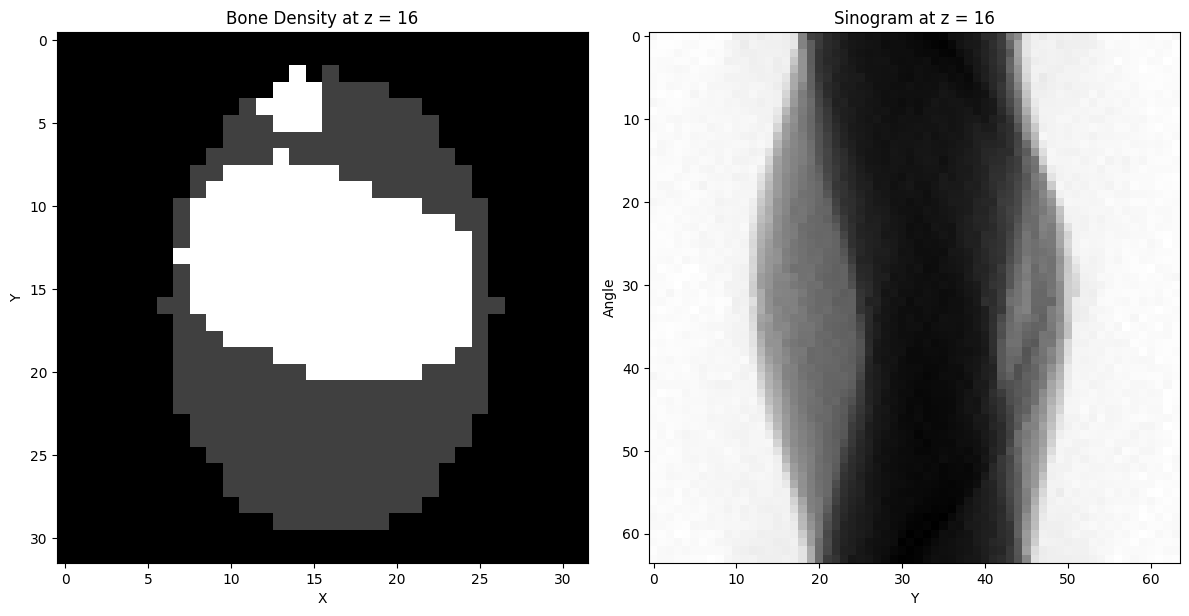
\includegraphics[width=0.7\linewidth]{files/a5464e97215c9d28832ba2f8c0a9a1da.png}
\caption[]{\textit{left:} a 2D slice of the phantom the colour gradient representing bone density. \textit{right} corresponding sinogram with 64 projection angles and a detector size in the y-direction of 64 pixels}
\label{phantomSinogram}
\end{figure}

The amount of photons detected can be plotted for each rotation angle as seen in Figure~\ref{phantomSinogram}, where the darker areas represent less photons detected at a y-level of the detector for a specific angle.

Recent breakthroughs in photon counting detectors make use of equation (\ref{muE}), where the linear attentuation coefficient depends on the energy level. The photon counting detectors (pcd) allow the classification of measured photons into energy bins \parencite{pcd2022}.

\subsection{Projection algorithms}

\begin{itemize}
\item brief overview backprojection  \parencite{zeng2001image}


\item list issues


\item brief overview itterative approach (with references to Mechlem)


\item positives


\item negatives
\end{itemize}

part of abstract: ``g. They require a specific
reconstruction process, consisting of two steps: material decomposition and tomographic
reconstruction. Image-based methods perform reconstruction, then decomposition, while
projection-based methods perform decomposition first, and then reconstruction. As an alternative,
`one-step inversion' methods have been proposed, which perform decomposition and reconstruction
simultaneously. Unfortunately, one-step methods are typically slower than their two-step
counterparts, and in most CT applications, reconstruction time is critical. This paper therefore
proposes to compare the convergence speeds of five one-step algorithms.'' \parencite{mory2018comparison}

itterative unet \parencite{ge2023mb}

\subsection{machine learning - CNN}

\begin{itemize}
\item How in image processing CNN have been used before \parencite{yamashita2018convolutional}


\item UNet github\parencite{ronneberger2015u}
\end{itemize}

\subsection{Machine learning - Attention}

\begin{itemize}
\item How we want to map the sinogram to the image, which is non-local \parencite{vaswani2017attention}
\end{itemize}

\section{Method}

\subsection{Data collection}

\begin{itemize}
\item pre existing algorithm
\item itterative steps
\item sinogram
\end{itemize}

\subsection{Pytorch}

\begin{itemize}
\item
\end{itemize}

\section{results}

\subsection{plot about speedup (time vs pixel size)}

either 2D or 3D

\subsection{plot about results for 32x32 simple phantom}

\subsection{plot harder phantom (3 features or more)}

\section{Discussion}

\subsection{non-machine learning speedup}

pytorch is highly optimized, mechlem is not

\subsection{pixel size and number of projections necessary}

There will not be a linear relationship between the amount of projections necessary and the amount of pixels in the image. will this have an impact?

\printbibliography

% DON'T EDIT. If "endfloat" option is enabled all floats appear before appendices
\if@endfloat\clearpage\processdelayedfloats\clearpage\fi


%%%%%%%%%%%%%%%%%%%%%%%%%%%%%%%%%%%%%%%%%%%%%%%%%%%%%%%%%%%%
%%% SUPPLEMENTARY MATERIAL / APPENDICES
%%%%%%%%%%%%%%%%%%%%%%%%%%%%%%%%%%%%%%%%%%%%%%%%%%%%%%%%%%%%
%% Sadly, we can't use floats in the appendix boxes. So they don't "float", but use \captionof{figure}{...} and \captionof{table}{...} to get them properly caption.

%%%%%%%%%%%%%%%%%%%%%%%%%%%%%%%%%%%%%%%%%%%%%%%%%%%%%%%%%%%%
%%% ARTICLE END
%%%%%%%%%%%%%%%%%%%%%%%%%%%%%%%%%%%%%%%%%%%%%%%%%%%%%%%%%%%%

\end{document}
